\section{Results}
%[PRG 10/9/15]
% incorporating andy's comments

Here we hope to understand the task-specific information provided by these visually responsive ring neurons by using simulation to investigate the outputs of sub-populations during well-known behavioural experiments (Figure~\ref{fig:recap}). In order to do this we use data from \citeA{Seelig2013} who used calcium imaging to examine the \acp{RF} of ring neurons whose cell bodies are in specific glomeruli in the lateral triangle. As the RFs of glomeruli are remarkably consistent across flies \cite{Seelig2013}, we can combine them across flies to reduce measurement error and obtain sets of `canonical' RFs. Though this averaging process will produce \acp{RF} that are more regular than those given for individual flies, this should not present a problem: for one, some of the irregularity in the \acp{RF} presumably derives from measurement error, and, for another, it seems unlikely that smoother edges on the \acp{RF} would give an `unfair advantage' in the tasks we are looking at.\todo{insertion}\ This process (for details, see Section~\ref{sec:methods:preprocessing}) gave us a set of 28 R2 and 14 R4d filters. Like mammalian simple cells \cite{Hubel1962,Wystrach2014CB}, the R2 and R4d ring neurons have RFs characteristic of bar and edge detectors (compare, e.g., R4d glom.~1 and R2 glom.~7 in Figure~\ref{fig:avkernels}D).
However, ring neuron RFs are coarser, covering a much larger region of the visual field, and are mostly tuned to orientations near the vertical (with a small number horizontally tuned). To investigate the information these cells encode, we calculate output values for a given visual stimulus by convolving it with the averaged ring neuron filters. This gives a population code whereby the outputs of the set of filters is the encoded `representation' of the current visual stimulus. We interrogate these encodings to understand the information they contain focusing on the relationships to specific behaviours.

%\subsection{Simulating the outputs of visually responsive ring neurons}
%%% dropped section, replaced by AP below

\subsection{Orientation towards bar stimuli}\todo{tweaked fig label as a couple of panels weren't mentioned + added stuff about why vector plot doesn't point to bar}
\label{sec:results:bar}
We first consider experiments in which flies are presented with bar stimuli.
As described above, flies will spontaneously orient towards black bars \cite{Gotz1987}.
More detailed assays show that flies will aim for the centres of narrow bars, and for the edges of wide bars \cite{Osorio1990}.
In our first analysis we examined the response of populations of simulated ring neurons to bars of different widths (Figure~\ref{fig:recap}A and B).
Looking at the raw summed output of the ensembles of ring neurons we see that activation profiles show peaks to the bars of different widths which broadly match experimental results (Figure~\ref{fig:recap}B).
For instance, R2 neurons respond maximally to the inside edges of large bars, which is where flies head when presented with wide vertical bars \cite{Osorio1990}, while peak activity in R4d neurons occurs at bar centres and also at roughly $\pm 90\degree$.
While we do not know the details of mechanisms downstream of the ring neurons and hence how the activity is transformed into behaviour, this modelling gives us an existence proof that the appropriate information is present in the sparse ring neuron code itself for the control of the observed behaviour. 

We further demonstrate this point by closing the loop between sensory systems and behaviour using a simple agent based model of a fly viewing a bar in which the fly's heading is controlled by the difference between the summed activation of left and right ring neurons (via a PID controller) (Figure~\ref{fig:recap}C). Our hypothetical agent approaches the bar from different distances, demonstrating bar fixation when far from a bar and fixation of the edges when nearer and the bar's apparent size is greater (Figure~\ref{fig:recap}D). Through this example, we can see how information present in even small populations of visually responsive ring neurons can control behaviour and more generally this shows how we can link outputs of sensory cells to a particular behaviour. We now turn to a more complex behaviour, pattern discrimination.

\subsection{Pattern discrimination in flies and ring neuron population codes}
\label{sec:results:pattern}

The standard paradigm for testing pattern discrimination in \emph{Drosophila} \cite{Dill1993,Ernst1999,Liu2006,Pan2009}, involves tethering a fly in a drum with a pair of alternating patterns on the inside wall of the drum (Figure~\ref{fig:recap}A).
When the fly attempts to rotate about the yaw-axis, the pattern on the drum is rotated by a corresponding amount in the opposite direction, giving closed-loop control.
Conditioning is aversive: orientation towards a quadrant containing one of the patterns of the pair is punished with heat from a laser.
Hence, if the fly can discriminate the patterns, it will eventually orient towards the non-punished pattern. The ability to discriminate patterns in such an assay requires R2 neurons, specifically synaptic plasticity afforded by \emph{rutabaga} in these neurons is sufficient and necessary \cite{Ernst1999,Liu2006,Wang2008,Pan2009}. Through analogy to artificial neural networks, we can relate flies' ability to learn to discriminate patterns to changing the output weights of the R2 population code. 

To recreate the visual information perceived by flies in such experiments, we simulated a typical experimental flight arena with a fly tethered in the centre. We then examined the output of the ensembles of ring neurons for a fly rotating in the drum and looked at the difference in the activation code when facing the different patterns of a pair. Our logic is that if the codes were identical, it would be impossible for the patterns to be discriminated by interrogating the outputs alone. Similarly, the further the patterns are apart, the easier they could be to discriminate (Figure~\ref{fig:recap}F and G, see Section~\ref{sec:methods:replication} for details). Our difference measure is the \ac{rms} difference between ensemble outputs when the fly faces different azimuths in the drum. As can be seen in Figure~\ref{fig:recap}, comparing the ensemble output for a simulated fly oriented at 0\degree\ (i.e. view centreed on one pattern) and the ensemble output when the `fly' is oriented at other azimuths, we can see how the code changes. The difference to the view at 0degrees rises as the fly rotates in the drum, peaking as it faces the space in between the patterns and dropping to a minimum when facing the centre of the next pattern (Figure~\ref{fig:recap}F and G). For some pairs of patterns, there is still a difference between the codes when facing the centres of each pattern enabling their discrimination. However, if we displace the patterns vertically, we see that the difference between codes when the fly fixates each pattern drops, despite the fact that to us, the patterns still appear very different. Interestingly, the second pattern is also harder to discriminate for flies.

In this way, we can use the difference between ensemble codes when flies face either pattern to re-examine the discriminability of pattern pairs tested with flies.
If our simulation provides a good approximation of the visual information available to the pattern learning/discrimination systems of a fly, we should see a close relationship between the \ac{rms} difference in simulated R2 output for a pattern pair and the flies' ability to learn to discriminate that pattern pair.
We thus examined the difference in the outputs of the R2 filters between patterns from pairs drawn from \citeA{Ernst1999}.
Figure~\ref{fig:pattern} shows these \ac{rms} differences, with pattern pairs numbered according to the figure in which they appear in \citeA{Ernst1999}.
In general, within these groups, the pattern pairs for which flies show a significant learned discrimination \cite<in>{Ernst1999} have a greater \ac{rms} difference in R2 population activity.
[THIS IS WHERE WE PUT THE Rank sum test] All of the pattern pairs where flies show significant learning ($n=8$) have \ac{rms} differences in R2 activity above the overall average (Figure~\ref{fig:pattern}A and B), whereas 13 out of 18 patterns that flies found more difficult to learn had \ac{rms} differences below average.\footnote{There were nine pattern pairs for which a significance level was not given that were excluded.}
Looking across all pattern pairs, we find a significant correlation between the strength of the learning index reported for flies in \citeA{Ernst1999} and the \ac{rms} difference we found in R2 activation (Spearman's rank, $n=30, \rho=.420, p < .05$).

\begin{comment}
Sig:
above: 8; below: 0; eq: 0; not given: 0; tot: 8
------
NS:
above: 5; below: 13; eq: 0; not given: 1; tot: 19
------
Sig not given:
above: 3; eq: 3; below: 0; not given: 3; tot: 9
------
tot tot: 36
\end{comment}

\begin{figure}
\vspace{-1cm}
\centering
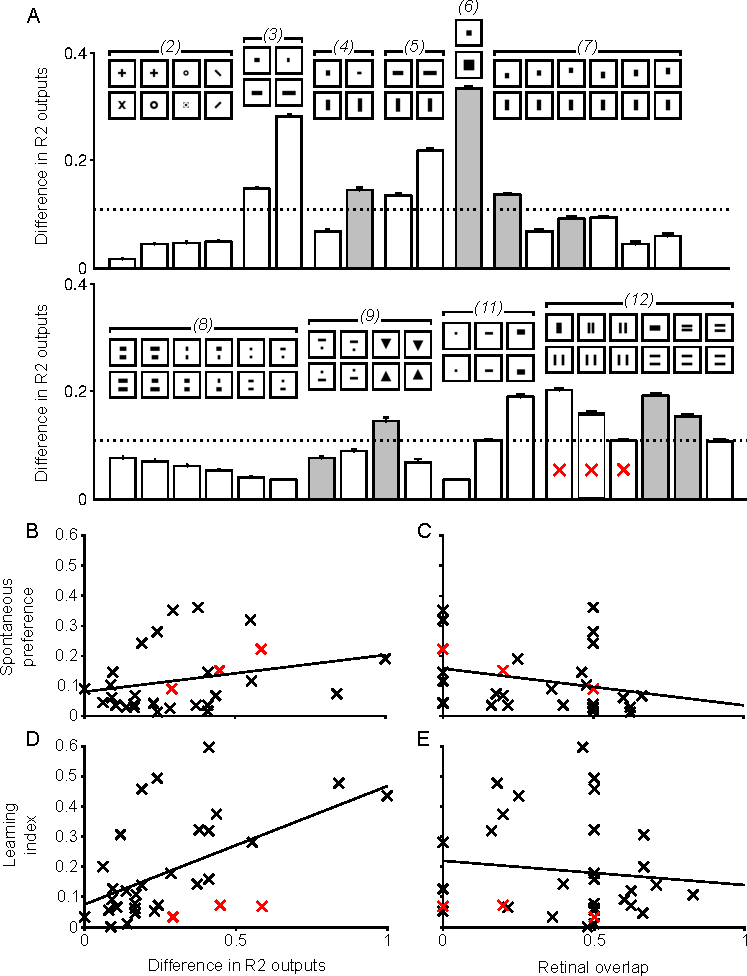
\includegraphics{figures/pattern}
\caption{[NB: I haven't put in the pattern pairs yet, but this should give an idea of the layout.]
Outputs of simulated R2 cells for published pattern pairs. Whether a pattern pair is discriminable by flies can be predicted partly on the basis of the difference in R2 activity.
The patterns tested here are drawn from \protect\cite{Ernst1999} and are grouped together according to the figures in which they appear in that work.
The corresponding figure numbers are shown in parentheses.
All patterns for which the significance of `learning preference' ($\overline{\mathrm{DCP}}$) was given are included.
Grey bars indicate that the $\overline{\mathrm{DCP}}$ for the pattern was significant ($p<.05$).
A higher score indicates a greater \ac{rms} difference in R2 activity and thus that the pattern was more discriminable by the simulation.
In general, within these groups, the patterns where there was a significant learned preference (in \protect\cite{Ernst1999}) have a greater difference in activity.
Performance on more `horizontal' patterns (e.g. \emph{(3)} and the final three patterns in \emph{(12)}) was poor in the behavioural experiments, but better in simulation.
This is perhaps due to the horizontal motion of the patterns in training, as noted in \protect\cite{Ernst1999}.
At the bottom are shown scatter plots of R2 difference (the `RF Model') and retinal overlap (the `Retinotopic Model') \emph{vs} learning index ($\overline{\mathrm{DCP}}$) shown in Ernst and Heisenberg \protect\cite{Ernst1999}.
The correlation for the RF Model was found to be significant (Spearman's rank, $n=34, \rho=.615, p<.005$), but not for the Retinotopic Model ($n=34, \rho= -0.215, p=\mathrm{n.s.}$).
}
\label{fig:pattern}
\end{figure}


Of course, these differences could simply result from the basic appearance of the patterns.
Therefore as a control comparison we also perform a parallel analysis where we quantify the similarity of patterns within a pair based on the degree to which the patterns overlap.
For this measure, there was no significant correlation with the flies' learning index over the pattern pairs (Spearman's rank, $n=32, \rho=-.068,p=\mathrm{n.s.}$).

We additionally looked at the relationship between our two visual encodings (R2 population code and the retinotopic encoding) and the degree to which flies' show a spontaneous preference for one of the patterns within a pair before any conditioning procedures have commenced (Figure~\ref{fig:pattern}D and E). For both retinotopic encoding and R2 population codes there was no significant correlation. This is in keeping with research showing that R2 neurons alone are critical for \emph{learned} pattern differences \cite{Ernst1999}, but not spontaneous preferences, which, by contrast, seem to result from activity across all subsets of ring neurons \cite{Solanki2015}.
We next discuss specific pattern sets in detail.

Set~\emph{(2)} in Figure~\ref{fig:pattern} gives examples of pattern pairs that are not discriminable by flies and also give only small differences in the outputs of R2 filters. This may seem surprising, given that these patterns appear quite different to human observers and are also very dissimilar if compared retinotopically. Thus we can see how the \emph{Drosophila} R2 ring neuron encoding is more informationally sparse. Whilst the human V1 region of human visual cortex contains neurons representing a full range of orientations all across the visual field, R2 neurons have large RFs and poor orientation resolution. Hence, a pattern pair consisting of a diagonal line facing left and a diagonal line facing right, for example, have only a small difference in R2 outputs in our simulation and are also not discriminable by flies.
This could, in the light of behavioural experiments alone, be interpreted as evidence that flies do not discriminate patterns on the basis of orientation.
A more parsimonious explanation, however, is that the flies are failing because the form of the \acp{RF} means that the activation triggered by each of the patterns is roughly the same.

Another illustrative example is Set~\emph{(9)}, which contains pairs of `triangles' (either a filled equilateral triangle, or a long and short bar arranged on top of one another), one facing up and the other down.
Flies are able to discriminate these pattern pairs when they are aligned along the top and bottom, but not when aligned about the vertical centres of mass \cite{Ernst1999}. Looking at the placement and form of the R2 RFs allows us to determine where this difference comes from (Figure~\ref{fig:simdiffpatts}).
The excitatory regions of the RFs fall roughly across the middle of triangles that are not aligned about their vertical centre of mass the difference in width at this point will lead to differences in activation. If the triangles are offset (Figure~\ref{fig:simdiffpatts}) so as to be aligned about their vertical centres of mass their width will be similar for the regions of peak R2 coverage and the difference in activation will be lower.
Thus the failure to be able to discriminate features with an equivalent vertical centre of mass can be explained by the shape of the RFs interacting with the patterns rather than the system somehow extracting and comparing the vertical centres of mass of the patterns.

\begin{figure}
\vspace{-3cm}
\centering
\includegraphics{figures/simdiffpatts}
\caption{
[PRG]
R2 cells do not encode detailed shape information.
A--C. The discriminability of pattern pairs can vary greatly independently of the apparent difference between visual stimuli. A. A pattern pair made up of a triangle and its inverse with both triangles aligned to their lowest points. B. The same triangles, but this time aligned by their centres of mass, make another pattern pair. C. The difference in activation between 0\degree\ and 90\degree\ for all R2 RF filters for the triangles from A (open bars)and B (closed bars). The mean activation difference is greater for the triangles in A over B. The red square marks the output of the ring neuron RF shown in A,B. 
D--F. We can also generate shapes that appear similar yet produce a large mean difference in RF activation (D) or appear different and produce similar RF activations (E). The stimuli here are `blobs' of the form described in Methods. An optimisation was performed in Matlab (\texttt{fminsearch} function) to minimise the ratio of blob difference to difference in activation (D) or its inverse (E). Pairs of stimuli are shown in grey and green whereas in the simulation both are black.
F. The corresponding activations of separate (left-hemispheric) R2 glomeruli are shown at the bottom. Two similar patterns give a mean difference in activity of 11.0\%. Two very different patterns give a mean difference in activity of 5.10\%.
}

\label{fig:simdiffpatts}
\end{figure}

We can further emphasise the independence of apparent similarity of patterns and the visual encoding from R2 cells, by designing shape pairs (Section~\ref{sec:methods:stimuli}) that appear similar to humans, but are easily discriminable to the R2 encoding (Figure~\ref{fig:simdiffpatts}D and white bars in F). Similarly, we can design shape pairs that are considered similar to the R2 network, but not to human observers (or retinotopic overlap algorithms) (Figure~\ref{fig:simdiffpatts}E and black bars F). Despite the similarity between the pairs of patterns, the first is readily discriminable especially from the outputs of glomeruli 1, 3, 5 and 11. In contrast the second pair -- which we easily see as having a different orientation -- have very low overall differences throughout the glomeruli. While this shows how we can get counterintuitive results due to the irregular RF shapes, being able to design shapes on the basis of the expected output of the R2 population could be a very useful tool in the design of future behavioural experiments.

There are, however, some discrepancies where the learning performance of flies for a pattern pair does not match the \ac{rms} difference of our R2 population code. In some cases flies are better at discriminating pairs of patterns that discriminate along the vertical rather than horizontal axis (Set~\emph{(3)} \emph{vs} Set~\emph{(4)}, and the pairs in Set~\emph{(12)}, marked with red Xs in Figure~\ref{fig:pattern}). In contrast, the \ac{rms} difference in the R2 population code discriminates horizontal and vertical patterns equally. This may be because while our R2 filters are being presented with static stimulus pairs to simulate a fly oriented to the centre of a pattern, for the flies the patterns were moving horizontally but fixed in the vertical axis \cite<as noted in>{Ernst1999} making it harder for flies to resolve horizontal information.

Overall, we have shown that the behavioural performance of flies on a pattern discrimination task is approximated by a simple difference metric applied to the R2 population activity of a small number of simulated R2 cells. Both flies and our R2 population are bad at a variety of seemingly simple pattern discriminations. A simple thought experiment is helpful in considering the purpose of the visual code provided by the small population of R2 neurons. If we double the number of R2 neurons in our population by inserting additional RFs of the same forms at random points on the visual field, then the \ac{rms} difference for centre of mass-aligned triangles increases to levels similar to those for pattern pairs easily discriminated by flies (data not shown). We can therefore see how the pattern discrimination ability of an R2-like neuronal population could easily have been improved over evolutionary time without need for any radical architectural changes, simply through the addition of more R2 cells. We propose that given how easily improved performance could have been achieved through evolution, there must be little selection pressure specifically for a specialised pattern recognition module in flies.

\subsection{What information is preserved in this simple neural code?}

Having such a small number of cells providing a visual encoding is essentially a sensory bottleneck with information from 3000 ommatidia condensed onto 28 R2 or 14 R4d ring neurons. We have shown above how this code provides sufficient information to discriminate some pattern pairs. However, general purpose pattern recognition seems unlikely to be a key visually guided behaviour for flies, as discrimination performance could be easily improved with the addition of more ring neurons in the R2 population. The question thus arises as to what information this system is tuned to extract. Examining the pattern pairs which flies and the R2 population were able to discriminate we see that certain pattern parameters are implicitly coded for in the R2 population. Sets~\emph{(6)} and \emph{(9)} (Figure xxx) suggest that shape size and vertical centre of mass are parameters that can be recovered from the R2 population code after the sensory bottleneck.

Here we therefore address in more general terms the shape information that may be implicitly conveyed in the ring neuron population code.
To do this, we generate large sets of blob-like patterns (see Section~\ref{sec:methods:stimuli}) that vary across a range of parameters (size, position, orientation). We then asked if an \ac{ANN} could be trained to recover this shape information from either a raw image of the shape (a control condition) or from the output of the R2/R4d population. Here we use ANNs as statistical engines interrogating the output of the ring neuron population code to determine the shape information that is implicit to the code and has therefore made it through the sensory bottleneck. 

We first examined whether ANNs could be trained to extract simple positional information (elevation and azimuth) about a stimulus from the ring neuron population codes. 
The stimuli used were ellipse-like `blobs', with orientation, $\theta$, and major-axis length, $a$, held constant ($\theta = 0\degree, a = 30\degree$).
There were 100 possible azimuths and 100 possible elevations, giving a total of 10,000 stimuli.
Of these, 4000 were used for training and 6000 for testing.
Results are shown in Figure~\ref{fig:elaz}.
We see that ANNs are indeed able to extract information about elevation and azimuth based on any of the input types.
Performance was better with parameter values near the middle, as at the extremes, portions of the stimuli lay outside the visual field of the simulated fly (see Figure~\ref{fig:elaz}A and B).
At the far extremes the stimuli begin to disappear `off the edge' of the visual field, making the task in principle a harder one (i.e., is it a large object projecting outside the visual field, or a smaller one just on the edge of the field of view?).\todo{added explanation of saturation effects}
Overall performance was best when ANNs were trained with raw views (Figure~\ref{fig:elaz}C and D). However ANNs also performed well with ring neuron inputs. The R2 code performs better than the R4d and it seems that the addition of R4d \acp{RF} to the R2 code, while adding much dimensionality, does not improve the performance, suggesting that either an R2-like encoding is sufficient to extract positional information, or that the information in the two codes is redundant. Thus we can see how very small populations of ring neurons retain simple positional information quite accurately.

\begin{figure}
\centering
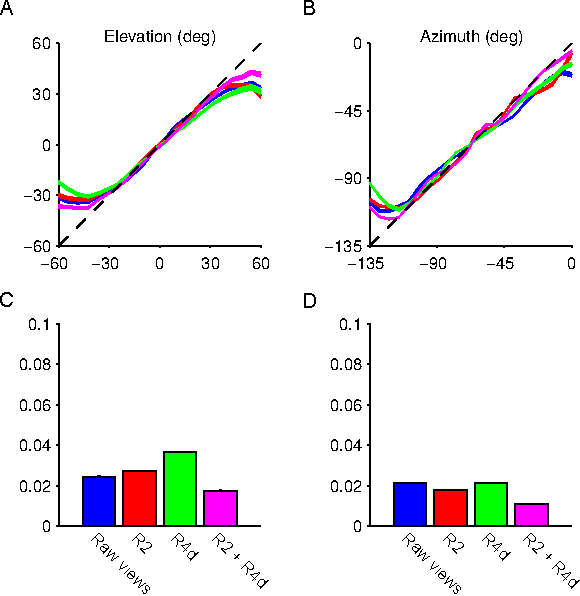
\includegraphics{drosopattern/elaz}
\thesiscaption{How much positional information is preserved in the R2 population code?}{
Neural networks were trained to estimate the elevation and azimuth of randomly generated `blob' stimuli ($N=10,000$)  from raw views ($N=36$~pixels; blue), R2 neurons ($N=28$; red), R4d neurons ($N=14$; green) or R2 and R4 neurons ($N=42$; magenta). For each visual input a network was trained 100 times and average performance with blobs that were not part of the training set was taken.
A and B: Plots of elevation and azimuth of the test visual stimuli \emph{vs} the mean network output ($N=100$). The dashed line indicates ideal performance (i.e. $y=x$) and the thickness of the lines at each point shows standard error.
The possible values of elevation and azimuth were constrained by the size of the fruitfly visual field (approx. $120\degree \times 270\degree$). Within this range there were 22 possible values.
C and D: Average network performance (mean square error) for networks trained to recover elevation (C) or azimuth (D) and for each type of visual input (colour code as above). Standard error is shown, but is very small.
}
\label{fig:drosopattern:elaz}
\end{figure}


We next trained the same kind of ANNs to decode information about shape orientation and size. The stimuli were again randomly generated ellipse-like blobs. Ten different orientations and sizes were used, giving a total of 1000 stimuli, of which 400 were used for training and 600 for testing. Figure~\ref{fig:orsi} shows how the ANNs were again able to extract this shape information from raw images and the sparse ring neuron codes. Orientation was the parameter with the highest error score, possibly because it fundamentally comes from a second-order statistic, the covariance of the shape. Nonetheless, both parameters could be simultaneously estimated by a neural network with ring neuron inputs, indicating that flies could be trained to distinguish arbitrary stimuli differing along these parameters.
(Interestingly, a network trained with all four of the parameters simultaneously -- elevation, azimuth, size and orientation -- had much more difficulty, particularly for orientation; data not shown.)

\begin{figure}
\centering
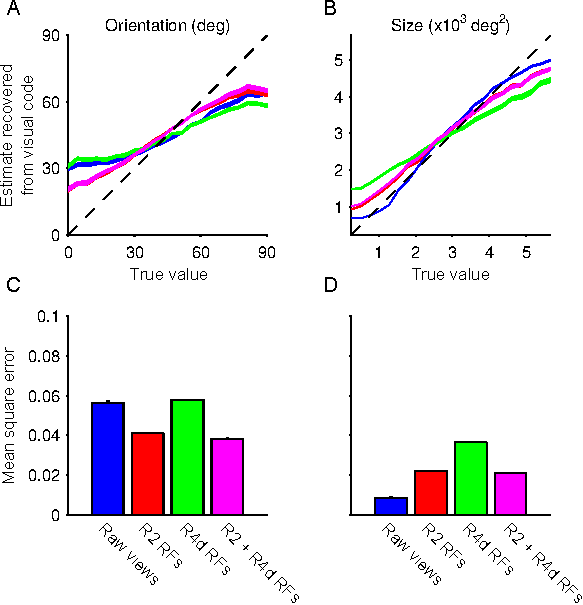
\includegraphics{figures/orsi}
\caption{How much shape information is preserved in the R2 population code?
Neural networks were trained to estimate the orientation and size of randomly generated 'blob' stimuli ($N=1000$) from different visual encodings (details same as for Figure~\ref{fig:elaz}).
A and B: Network performance in recovering stimulus orientation and size. Orientation was constrained between 0\degree\ and 90\degree, to avoid the problem of aliasing, and varied with 22 levels (conventions as in Figure~\ref{fig:elaz}).
C and D: Average network performance (mean square error) for networks trained to recover orientation (C) or size (D) and for each type of visual input (colour code as previously). Standard error is shown, but is very small.
}
\label{fig:orsi}
\end{figure}


In summary, we have shown that information about a number of shape properties passes through the bottleneck created by the small number of ring neurons.
This indicates that such information is available downstream of the ring neurons for the guidance of behaviour.
